\chapter{Circular Motion}

\section{Angular Displacement and Velocity}

\begin{definition}
    For a particle moving over an arc of a circle, its \vocab{angular displacement} ($\t$) is the directed angle subtended by the arc at its centre.
\end{definition}

Its SI unit is the radian (rad).

Equivalently, the angular displacement $\t$ due to an arc of length $s$ and radius $r$ is given by \[\t = \frac{s}{r}.\]

\begin{definition}
    \vocab{Angular velocity} ($\o$) is the rate of change of angular displacement. \[\o = \der{\t}{t}.\]
\end{definition}

Its SI unit is radian per second (rad s$^{-1}$).

\begin{proposition}
    Assuming the radius of the arc $r$ is constant, the linear velocity $v$ and the angular velocity $\o$ are related by \[v = r \o.\]
\end{proposition}
\begin{proof}
    We have \[v = \der{s}{t} = \der{(r \t)}{t} = r \der{\t}{t} = r\o.\]
\end{proof}

The direction of the linear velocity is tangential to the circular path.

\begin{figure}[H]
    \centering
    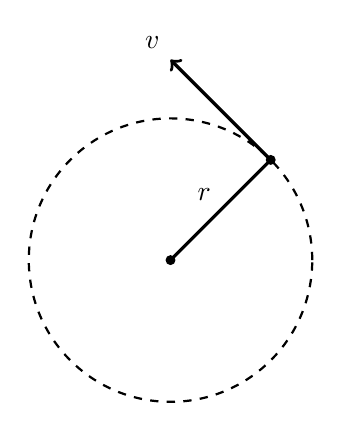
\begin{tikzpicture}[scale=0.6]
        \draw[thick, dashed] (0, 0) circle[radius=3];
        \fill (0, 0) circle[radius=3pt];
        \fill (2.121, 2.121) circle[radius=3pt];
        \draw[->, very thick] (0, 0) -- (2.121, 2.121) -- (0, 4.242) node[anchor=south east] {$v$};
        \node[anchor=south east] at (1.061, 1.061) {$r$};
    \end{tikzpicture}
    \caption{$v$ is tangent to the circular path.}
\end{figure}

\section{Uniform Circular Motion}

\begin{definition}
    When the angular velocity of a body is constant, the body is said to be moving in \vocab{uniform circular motion}.
\end{definition}

In uniform circular motion, we simply have \[\o = \frac{\t}{t}.\]

\begin{definition}
    A body moving in a circular path with constant speed is said to be in \vocab{uniform circular motion}.
\end{definition}

\subsection{Centripetal Acceleration}

\begin{definition}
    \vocab{Centripetal acceleration} ($a$) is the acceleration of a body in uniform circular motion.
\end{definition}

Its SI unit is metres per second squared (m s$^{-2}$).

Since the magnitude of the body's velocity is constant, the centripetal acceleration only changes the direction of the velocity. Hence, it is perpendicular to the direction of travel, i.e. it points towards the centre of the circular path.

\begin{figure}[H]
    \centering
    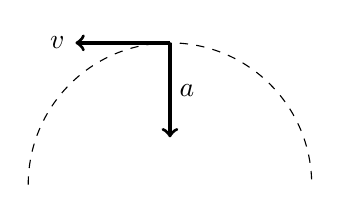
\begin{tikzpicture}[scale=0.6]
        \draw[dashed] (-3, 0) arc (180:0:3);

        \draw[->, very thick] (0, 3) -- (-2, 3) node[anchor=east] {$v$};
        \draw[->, very thick] (0, 3) -- (0, 1);
        \node[anchor=west] at (0, 2) {$a$};
    \end{tikzpicture}
    \caption{The centripetal acceleration $a$ of a particle in uniform circular motion.}
\end{figure}

\begin{proposition}
    The centripetal acceleration $a$ of a body in uniform circular motion is given by \[a = \frac{v^2}{r} = r\o^2 = v\o.\]
\end{proposition}
\begin{proof}
    Imagine an object steadily traversing a circle of radius $r$ centred on the origin. Its position can be represented by a vector of constant length that changes angle. The total distance covered in one cycle is $2\pi r$. This is also the accumulated amount by which the position has changed.

    Now consider the velocity vector of this object: it can also be represented by a vector of constant length that steadily changes direction. This vector has magnitude $v$, so the accumulated change in velocity is $2\pi v$.

    The magnitude of acceleration is then \[a = \frac{\text{change in velocity}}{\text{time elapsed}} = \frac{\text{change in velocity}}{\text{total distance travelled} / \text{speed}} = \frac{2\pi v}{2\pi r / v} = \frac{v^2}{r}.\]
\end{proof}

\subsection{Centripetal Force}

\begin{definition}
    \vocab{Centripetal force} ($F$) is the force producing the centripetal acceleration.
\end{definition}

\begin{proposition}
    The centripetal force is given by \[F = m \frac{v^2}{r} = m r \o^2 = m v \o.\]
\end{proposition}
\begin{proof}
    From Newton's second law, we know that for an object with constant mass $m$, we have $F = ma$. But $a = v^2/r = r\o^2 = v\o$, so \[F = m \frac{v^2}{r} = m r \o^2 = m v \o.\]
\end{proof}